\documentclass[a4paper, 11pt]{report}
\usepackage{blindtext}
\usepackage[textwidth=14.5cm]{geometry}
\usepackage[T1]{fontenc}
\usepackage[utf8]{inputenc}
\usepackage{titlesec}
\usepackage{fancyhdr}
\usepackage{geometry}
\usepackage{graphicx}
\usepackage[rightcaption]{sidecap}
\usepackage{enumerate}
\usepackage[english]{babel}
\usepackage[style=apa6,sortcites=true,sorting=nyt,backend=biber]{biblatex}
\addbibresource{info1111-group-project.bib}
\DeclareLanguageMapping{american}{american-apa}
\usepackage{csquotes}
\usepackage{lmodern}
\setcounter{biburlnumpenalty}{9000}
\parindent=0pt

\geometry{ margin=30mm }
\counterwithin{subsection}{section}
\renewcommand\thesection{\arabic{section}.}
\renewcommand\thesubsection{\thesection\arabic{subsection}.}
\usepackage{tocloft}
\renewcommand{\cftchapleader}{\cftdotfill{\cftdotsep}}
\renewcommand{\cftsecleader}{\cftdotfill{\cftdotsep}}
\setlength{\cftsecindent}{2.2em}
\setlength{\cftsubsecindent}{4.2em}
\setlength{\cftsecnumwidth}{2em}
\setlength{\cftsubsecnumwidth}{2.5em}


\begin{document}\sloppy
\titleformat{\section}
{\normalfont\fontsize{15}{0}\bfseries}{\thesection}{1em}{}
\titlespacing{\section}{0cm}{0.5cm}{0.15cm}
\titleformat{\subsection}
{\normalfont\fontsize{13}{0}\bfseries}{\thesubsection}{0.5em}{}
\titlespacing{\section}{0cm}{0.5cm}{0.15cm}

%=======================================================================================

\begin{titlepage}
\center 
\textbf{\huge INFO1111: Computing 1A Professionalism}\\[0.75cm]
\textbf{\huge 2022 Semester 1}\\[2cm]
\textbf{\huge Practice: Team Project Report}\\[3cm]

\textbf{\huge Submission number: ??}\\[0.75cm]
\textbf{\huge Team Members:}\\[0.75cm]
\textbf{\large
    \begin{tabular}{|p{0.5\textwidth}|p{0.3\textwidth}|p{0.2\textwidth}|}
        \hline
        Name & Student ID & Levels being attempted in this submission\\
        \hline
        Xiyan Huang & 510221401 & 2 \\
        ?? & ?? & ?? \\
        ?? & ?? & ?? \\
        ?? & ?? & ?? \\
        \hline
    \end{tabular}
}\\[0.75cm]
\end{titlepage}

%=======================================================================================

\tableofcontents

%=======================================================================================

\newpage
\section{Level 1: Basic Skills}

\subsection{Developing industry skills}

\subsubsection{Online Interactive Platform}

\subsubsection{Online Course}

\subsubsection{Official Documentation}

\subsubsection{Discussion Platform}

\paragraph{Example}
CSDN is one of China's most comprehensive information technology communities and service platforms. Every day, over 100,000 people converse and exchange expertise and information via CSDN's Web forums, which have almost 50 million registered members. \cite{(Xing et al., 2019)}\\

\paragraph{Pros}
People are increasingly interested in community question answering (CQA) websites because of their ability to solve various problems. A rapid increase in the number of users of these networks has been seen in recent years. The popularity of these networks may be shown by looking at the traffic on famous CQA sites like StackOverflow, Quora, and Yahoo! Answers. CQA websites now provide users with an excellent platform for sharing and finding information, thanks to the rising amount of data. Users can participate and engage by asking and answering questions, leaving comments, voting, etc. They can also indicate the best response among offered replies in various CQAs, such as StackOverflow, which introduces the idea of an approved answer. \cite{(Dargahi Nobari et al., 2020)} For a programming learner, it can help your practical problem such as "Why do I get this exception as my output?" when you post it or take a look at other's post where they have the same problem as yours and others solved it their question. Therefore, the discussion platform is quite helpful for actual problem-solving.\\

\paragraph{Cons}
The users who can offer high-quality answers to the more hard questions submitted in the community are critical to the success of CQA systems. \cite{(Dargahi Nobari et al., 2020)} Therefore, the quality and correctness of the solutions in the platform are still a thoughtful thing. Much research has been conducted in recent years to address expertise retrieval as a superior Information Retrieval (IR) task, a well-established topic in IR, and challenging work. \cite{(Dargahi Nobari et al., 2020)} The developers of the discussion forum still have a lot of things to do in the long run.
\subsubsection{Textbooks}

%=======================================================================================

\newpage
\subsection{Skills: add student 1 name here : Computer Science}



%=======================================================================================

\newpage
\subsection{Xiyan Huang : Data-science}

 \begin{figure}[t]
   \caption{\cite{(Conway, 2010)}}
      \centering
      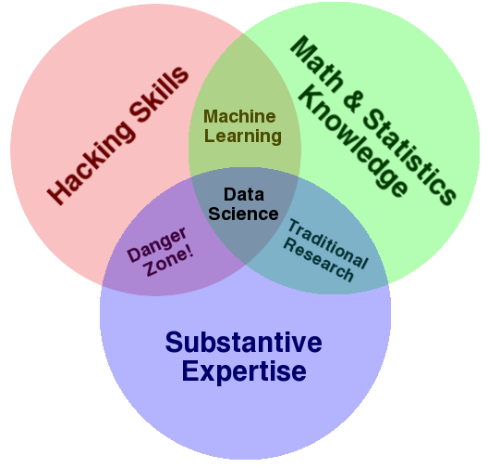
\includegraphics[width=0.5\textwidth]{Data-science}
   \end{figure}

While some of the junction labels are a little sarcastic, I believe this graphic captures the heart of what I think people mean when they say "data science": it is inherently an interdisciplinary field. The skills of a statistician who knows how to model and summarize datasets; the skills of a computer scientist who can design and use algorithms to efficiently store, process, and visualize this data; and the domain expertise—what we might think of as "traditional" training in a subject—necessary both to formulate the right questions and to put their answers in context. \cite{(Vanderplas, 2017)} There are some kinds of skills below that are considered the most useful ones in our future learning.\\

\subsubsection{Mathematical skills}
From my perspective, mathematics, predominantly linear algebra, calculus, probability and statistics, are pretty crucial for future learning. Math helps us better understand the principle behind the formula and the code we use.\\
\paragraph{Linear algebra}
Linear algebra is an area of mathematics that comes in handy for data science and machine learning. The majority of machine learning models may be written as a matrix, a typical dataset representation. Data preparation, data transformation, and model assessment all involve linear algebra. \cite{(Benjamin Obi Tayo, Ph.D., 2021)}\\
\paragraph{Calculus}
In machine learning models, calculus and optimization are used to arrive at the final answer. When creating a suitable algorithm model, the final solution frequently includes an optimization problem. Without the help of differential theory and calculation methods, no elegant model can be produced in the process of exploring the extremes of data space. As a result, the only approach to the final answer is to grasp the basic idea of multivariate differentiation and the optimization realization technique. \cite{(Zhang, 2020)}\\
\paragraph{Probability}
Probability statistics is a technique for deducing rules from data and speculating on the unknown. \cite{(Zhang, 2020)}. Probability is crucial for hypothesis testing and distributions like the Gaussian distribution and probability density function. \cite{(Ronald Van Loon, 2020)}\\
\paragraph{Statistics}
Statistics are at the heart of advanced machine learning algorithms in data science, capturing and translating data patterns into actionable evidence. Data scientists use statistics to collect, review, analyze, and draw conclusions from data and apply quantified mathematical models to appropriate variables. Data scientists operate in various capacities, including programmers, academics, and corporate executives. However, there is one thing that all of these fields have in common: a statistical foundation. \cite{(How Much Do Data Scientists Need to Know about Statistics?, 2021)}\\
\subsubsection{Python skills}
Python remains a really valuable tool in my opinion. Pythonistas have contributed a large number of modules, packages, and contributions to the rest of the community, making it a valuable programming language to learn. \cite{(Rogel-Salazar, 2020)} Python has established itself as a first-class tool for scientific computing activities, such as analysing and visualising massive datasets, during the previous two decades. This may have surprised early Python proponents, given the language was not built with data analysis or scientific computing in mind. NumPy for manipulating homogeneous array-based data, Pandas for managing heterogeneous and labelled data, SciPy for everyday scientific computing tasks, Matplotlib for publication-quality visualisations, IPython for interactive execution and sharing of code, Scikit-Learn for machine learning, and many more tools will be discussed in the following sections. \cite{(Vanderplas, 2017)}\\
\subsubsection{R skills}
R is linked to a statistics-focused computer environment, where many innovative techniques in genetics and biomedicine are initially published. \cite{(Pittard & Li, 2020)} One of R's most significant features is that it is open-source, which means that anybody may access the underlying code that runs the program and modify it for free. That is to say, R: will always be able to execute the most up-to-date statistical analyses as soon as they are thought of; will swiftly and transparently correct any flaws; and has gathered a community of programming and statistics geeks (a.k.a., useRs) to whom you may turn for assistance. Furthermore, anybody may examine the code in a package. R can overcome many obstacles to doing reproducible research on a global scale. R is rapidly being utilized as an industry standard in data analytics, sometimes known as "data science," which is another reason you should become a useR. Many organizations that hire psychology PhD students (e.g., Facebook, Merck, Pfizer) look for robust statistics and programming applicants. If you apply for nonacademic positions, learning R will make you a more appealing candidate, and teaching R will provide your students with additional career alternatives. \cite{(Yee, 2017)}\\
\subsubsection{Git skills}
Even if no software development is involved, version control is essential for managing large projects. Git is a distributed paradigm that allows developers to "clone" repositories, including any related change history, and submit changes for (re)integration into the reference copy, sometimes known as the "main branch." Git can help discover and resolve conflicts in which many persons modify the same file. It's perfect for organizing massive, dispersed projects with hundreds of participants, but it's also suitable for laboratory-based informaticists writing code for a publication. Git is language-neutral, seeing source code as plain text files that must be checked for changes. The functionality of Git is independent of the programming language used. \cite{(Pittard & Li, 2020)}\\
\subsubsection{Docker skills}
Every software program of real-world complexity will rely on other applications and libraries to work. These programs and libraries will also depend on computer environments, including operating system functions. Some of them may be limited to specific operating systems. Virtual machines can allow access to several operating systems without requiring the purchase of a new computer. VirtualBox, for example, enables Linux to operate on a local Windows machine. Another reason to use containers is the issue of program dependence and compatibility, which is possibly more relevant in data science. A software application's libraries will evolve, have several versions, and some will become obsolete after a while. As a result, software applications that rely on specific libraries frequently breaks, failing to execute. The approach is to record the exact versions and copies of these libraries that the software program is designed to run. Although a virtual machine image may be created for this, containers are the way to do it regularly as part of a daily routine. Containers simplify the installation and deployment of software applications in practice. \cite{(Pittard & Li, 2020)}\\
\subsubsection{Collaborating skills}
\paragraph{Discipline}
Data science is a team, not a single person. The importance of diversity cannot be overstated. Statisticians, data engineers/computer scientists, machine learning optimisers, and subject matter experts are all needed. It also requires curiosity about issues, recognising and presenting difficulties to address them; investigative and problem-solving skills; data collection, data problem-solving, and technical skills; and a challenge team. \cite{(MacGillivray, 2019)}\\
\paragraph{Interdiscipline}
On the other hand, interdisciplinary collaboration entails integrating knowledge from two or more fields. Participants often come from several disciplines and collaborate to develop new understanding by combining information from their respective fields. \cite{(Blaise Cronin, American Society For Information Science And Technology, and Information Today, Inc, 2007)} for example, as a data science student, we can collaborate with computer science student to better our programming skills, business student to get fund for our project, and math student analysis to promote out althogorithm.\\
\subsubsection{Research skills}
Despite the importance of research methodologies and statistics training for social work students, these courses frequently fail to meet the demands of organizations in collecting, organizing, and using data for data-driven decision making. For example, according to the data science literature, acquiring, maintaining, and preparing data for analysis consumes 80\% of the resources for data initiatives. \cite{(Perron, Victor, Hiltz, & Ryan, 2020)} The skills for data acquisition, data preparation, data usage and data governance are essential when dealing with big data. Data acquisition is extracting or getting existing data but stored to prevent it from being analysed right away. Cleaning, converting, combining, and connecting data files are just a few of the activities that make existing data useable. Data consumption allows for more options to provide personalised data to the end user's information demands. Data governance refers to a company's policies and procedures for managing data across the data life cycle. \cite{(Perron, Victor, Hiltz, & Ryan, 2020)}\\
\subsubsection{Structured Query Language skills}
The de facto standard language for manipulating and retrieving data from relational databases is SQL. A programmer or database administrator with SQL can change the structure of a database, change the security settings on your computer, add user permissions to databases or tables, obtain information from a database by querying it, and update a database's contents. The program can connect to a database on a distant server using SQL and a network connection. Because of the improved capability of personal computer hardware, crucial database information may now be housed on a low-cost standalone server. Furthermore, the client apps may be changed with little or no modification to the server. One of SQL's most significant advantages is a cross-platform and cross-product language. Because it is also referred to as a high-level or fourth-generation language (4GL) by programmers, it allows for the completion of a tremendous amount of work with fewer lines of code. \cite{(Stephens & Plew, 2003)}\\

%=======================================================================================

\newpage
\subsection{Skills: add student 3 name here : Software Development}

Your text goes here

%=======================================================================================

\newpage
\subsection{Skills: add student 4 name here : Cyber Security}

Your text goes here


%=======================================================================================

\newpage
\section{Level 2: Basic Technology}

\subsection{Tech Stack: Xiyan Huang}

\subsubsection{MERN introduction}
The MERN (MongoDB, Express, React.js, Node.js) stack was one of the first open-source stacks to embrace SPAs and NoSQL. This stack was anchored by React.js, a JavaScript library for building user interfaces, so in some sense, it’s the View part of the Model View Controller (MVC) architectural paradigm. For durable data storage, MongoDB, a popular NoSQL database, was employed. The middle-tier, or web server, was made up of Node.js, a server-side JavaScript runtime environment, and Express, a Node.js-based web server. Until a few years ago, this stack was perhaps the most popular for any new online application.\cite{(Vasan Subramanian, 2019)}\\

 \begin{figure}[t]
   \caption{\cite{(MongoDB, n.d.)}}
      \centering
      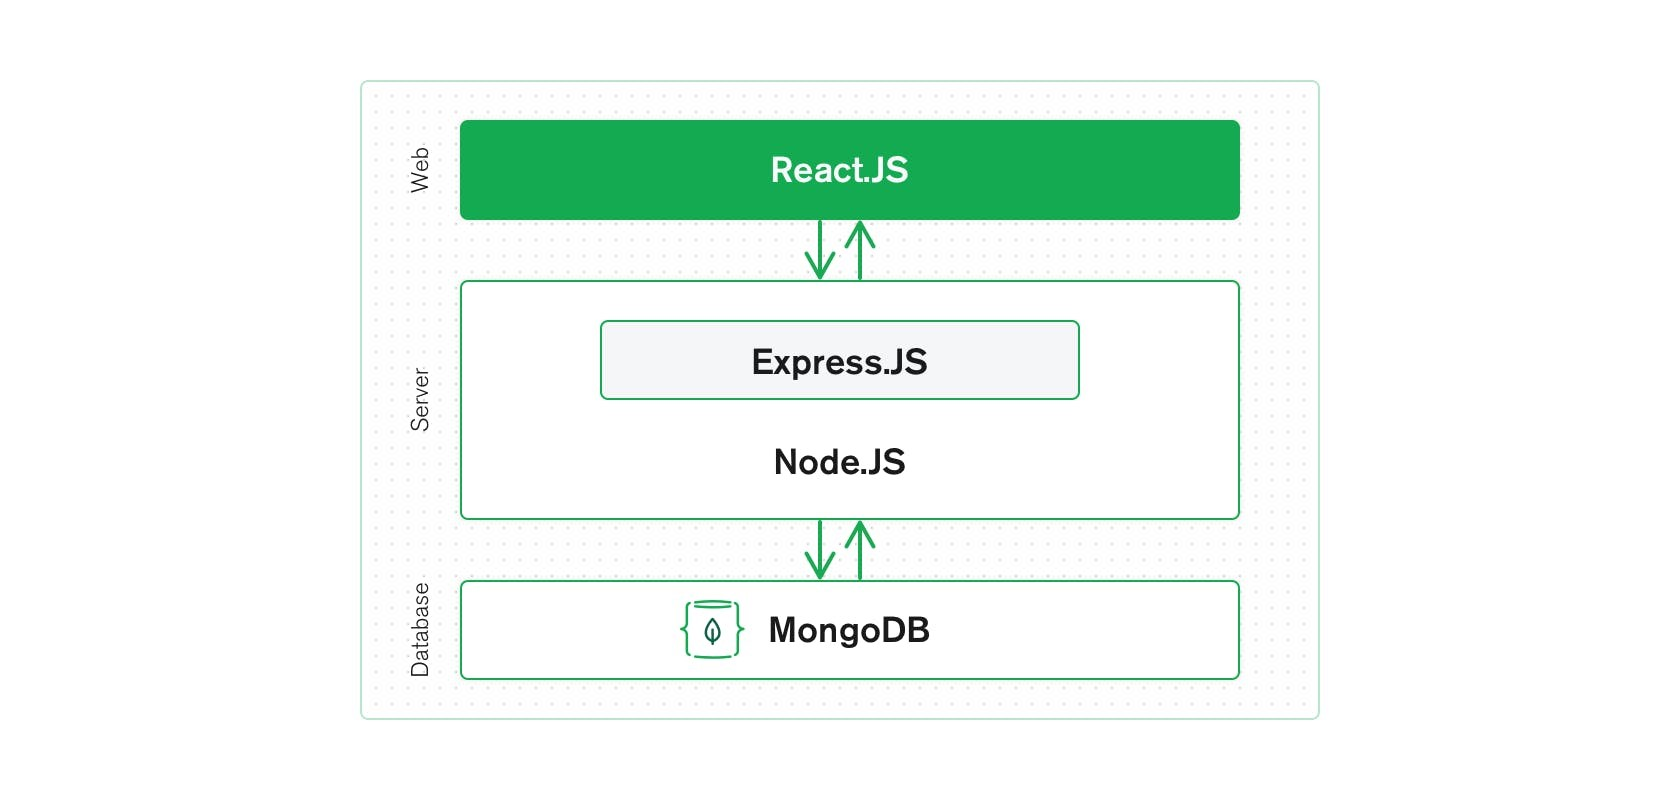
\includegraphics[width=0.6\textwidth]{MERN}
   \end{figure}

\paragraph{Front End} 
React.js, a declarative JavaScript framework for generating dynamic client-side apps in HTML, sits at the top of the MERN stack. \cite{(MongoDB, n.d.)} React is a JavaScript library that presents data as HTML views and is a free source. It has the properties of simplicity, continuity, and integration. For simplicity, react provides a simple API that can be picked up quickly. Even big apps are easy to comprehend and intelligible because React's an architectural paradigm that keeps the application state centralized and data flowing only in one direction. For its continuity, changes to the React API are being introduced with caution. Incompatible updates are adequately notified in advance, and APIs are only shut down when a successor is available. For the integration part, since React is only a view framework, you have complete control over how and with which approaches you to create the rest of your project. Because React makes minimal assumptions about its surroundings, it works well with existing applications and enables easy conversion. \cite{(Zeigermann & Hartmann, 2016)}\\

\paragraph{Server Tier}
The Express.js server-side framework, which runs within a Node.js server, is the next step down. Express.js describes itself as a "quick, unopinionated, minimalist web framework for Node.js," and it is precisely that. Express.js, or Express for short, is a Node.js Web application framework released under the MIT license as free and open-source software. It's made for creating Web apps and APIs. It has established itself as the de facto standard for Node.js server frameworks. Node.js is a cross-platform execution environment that can run JavaScript on the server and is open source.Node.js comes with several fundamental modules pre-installed. These modules provide you access to the file system, networking, input/output, and other aspects of the operating system. They also offer various utility functions that almost all applications require. \cite{(Vasan Subramanian, 2019)}\\

\paragraph{Database Tier}
MongoDB is a general-purpose database that is powerful, versatile, and scalable. It combines capabilities like secondary indexes, range queries, sorting, aggregations, and geographic indexes with the capacity to scale out. \cite{(MongoDB, n.d.)} Apart from producing, reading, updating, and removing data, MongoDB includes unique, compound, geographic, and full-text indexing capabilities and general secondary indexes that enable a range of quick searches. MongoDB has an "aggregation pipeline" feature that lets you create complicated aggregations out of essential bits and let the database optimize them. Time-to-live collections, such as sessions, are supported by MongoDB for data that should expire at a specific time. Fixed-size exhibitions are also supported, handy for storing current data such as logs. MongoDB has a simple mechanism for storing huge files and their information. \cite{(Bradshaw, Chodorow, & Eoin Brazil, 2019)}\\

You may connect to Express.js functions that power your application by sending XML HTTP Requests (XHRs), GETs, or POSTs from your React.js front-end. To access and change data in your MongoDB database, those methods use MongoDB's Node.js drivers, either via callbacks or Promises. \cite{(MongoDB, n.d.)}

\subsubsection{MERN Advantages}
MongoDB, the MERN stack's document database, was created from the ground up to store JSON data natively. Everything from its command-line interface to its query language is based on JSON and JavaScript.MongoDB and Node.js work together flawlessly, making it simple to store, modify, and express JSON data at all application levels. With only a few button clicks, MongoDB Atlas provides an auto-scaling MongoDB cluster on the cloud provider of your choosing, making cloud-native apps easy. Express.js (which runs on Node.js) and react.js are part of the JavaScript/JSON application MERN's entire stack. Js is a server-side application framework that covers HTTP requests and responses and makes mapping URLs to server-side actions a breeze. Js is a front-end framework for building dynamic HTML user interfaces that connect with distant servers using JavaScript.\\

JSON data may quickly move from the front end to the back end due to this combination, making development and debugging faster. Furthermore, mastering the system necessitates a thorough understanding of a programming language and the JSON document format! \cite{(MongoDB, n.d.)}\\

Like MEAN, it uses JavaScript as the primary programming language and runs at every application level. It makes it very efficient and helps developers follow modern Web development methods. MERN is also open source and has strong support from the global developer community. It also supports model View Controller (MVC) architecture to make the development process smoother with various programming languages. It uses Node.js, which is fast and efficient due to its asynchronous nature. If we compare it to other languages, its performance is excellent. React is great for front-end development, providing an unparalleled experience for the end-user. Some well-known sites, like Facebook, Dropbox, and Airbnb, use React to create unique user interfaces.\\

\subsubsection{MERN Disadvantages}
While React offers a groundbreaking interface and experience, developers face hurdles because it is a library rather than a mature framework with limited core features. Therefore, developers must rely on third-party services. It does not support direct calls to interact with the back-end server. It is not recommended for large-scale applications.\cite{(Mathur, 2020)}

\subsubsection{MERN Applications}
\paragraph{E-Commerce Applications}
Because of its MVC framework and outstanding possibilities like authentication, easy authorization, ORMs, and so on, MERN is chosen for eCommerce development.\\
\paragraph{CRM or Customer Relationship Management System Applications}
LinkedIn employs the MERN stack to let users sign in with their LinkedIn credentials via a quick and simple mobile application.\\
\paragraph{Build a Cross-Platform Mobile Game}
Because hybrid app development using the Ionic framework is rapidly gaining popularity, now is a beautiful moment to design a cross-platform mobile game.\\
\paragraph{Data Visualization}
React.js and Node.js are used by iCharts, the most popular stock market data platform, to show data in an aesthetically pleasing manner with easy navigation.\\
\paragraph{Personal Websites or Blogs}
Due to its full-stack framework integrating React.js at both the frontend and backend levels, MERN is the ideal solution if your website needs to manage traffic. It has a lot of scalabilities.\cite{(Kapoor, 2021)}\\

%=======================================================================================

\newpage
\subsection{Tech Stack: add student 2 name here}

Your text goes here

%=======================================================================================

\newpage
\subsection{Tech Stack: add student 3 name here}

Your text goes here

%=======================================================================================

\newpage
\subsection{Tech Stack: add student 4 name here}

Your text goes here


%=======================================================================================

\newpage
\section{Level 3: Advanced Skills}

Level 3 focuses on more advanced technical skills (\LaTeX\ and Git) and analysis of linkages and relationships between the items in the company tech stack.

The following is a list of advanced Git and \LaTeX\ skills/features. Each student should select one pair of items from each list and demonstrate actual use of each item (either through activity in Git, or through including items in this report). (Target = $\sim$100 words per student for each feature).
\begin{itemize}
    \item Git
    \begin{itemize}
        \item Rebasing and Ignoring files
        \item Forking and Special files
        \item Resetting and Tags
        \item Reverting and Automated merges
        \item Hooks and Tags
    \end{itemize}
    \item \LaTeX\ 
    \begin{itemize}
        \item Cross-referencing and Custom commands
        \item Footnotes/margin notes and creating new environments
        \item Floating figures and editing style sheets
        \item Graphics and advanced mathematical equations
        \item Macros and hyperlinks
    \end{itemize}
\end{itemize}

\subsection{Advanced features: add student 1 name here}

Explain your use of the advanced Git and \LaTeX\ features. 

\subsection{Advanced features: add student 2 name here}

Explain your use of the advanced Git and \LaTeX\ features. 

\subsection{Advanced features: add student 3 name here}

Explain your use of the advanced Git and \LaTeX\ features. 

\subsection{Advanced features: add student 4 name here}

Explain your use of the advanced Git and \LaTeX\ features. 



%=======================================================================================

\newpage
\section{Level 4: Advanced Knowledge}

Level 4 focuses on analysing your particular tech stack and considering alternatives. Each student should consider the tech stack they described for Level 2, and then discuss each of the following points:
\begin{itemize}
    \item What are the strengths and limitations of this stack? (Target = $\sim$200 words).
    \item What alternatives exist, and under what situations might these alternatives be a better choice? (Target = $\sim$200 words).
\end{itemize}

\subsection{Advanced Knowledge: add student 1 name here}

Your text goes here

\subsection{Advanced Knowledge: add student 2 name here}

Your text goes here

\subsection{Advanced Knowledge: add student 3 name here}

Your text goes here

\subsection{Advanced Knowledge: add student 4 name here}

Your text goes here



%=======================================================================================

\newpage

\printbibliography

\end{document}
\end{report}
